
\chapter{Context}

\begin{figure}[htb]
\begin{center}
\leavevmode
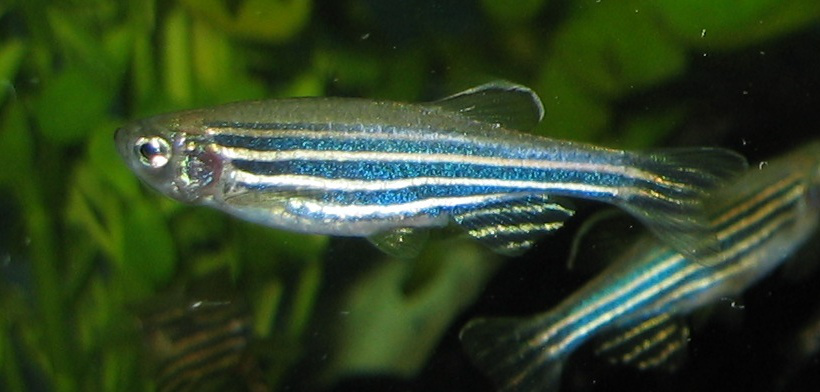
\includegraphics[width=0.99\textwidth]{pictures/zebrafishPic}
\end{center}
\caption{Mature zebra fish: approximatively 2.5cm long (source: \href{http://en.wikipedia.org/wiki/File:Zebrafisch.jpg}{Wikipedia})}
\label{fig:ZebraPic}
\end{figure}

\section{Systems Biology}

With the completion of the genome projects~\cite{}, the stage is now set for a
more complete understanding of how animals are created. Biologists now have
access to the complete sequence of DNA that encodes the blueprint of life for
many animals including human, mouse, zebrafish, and fruit
fly~\cite{[2][3][4][5]} \TODO{refe?}The challenge is now understanding how this
code functions. The problem however is that the only thing that biologists can
currently reliably predict from the genomic code is which parts can be
transcribed and translated into protein. Biologists cannot accurately predict
when and where a protein will be expressed, how a protein will
function once it is created, and the interaction between expressed proteins that
allow them to form functional genetic circuits. Thus, although the genome
projects have given us the complete code for constructing many organisms, the
only part of the code biologists can currently read is the parts list. The
challenge is understanding how all these parts fit together to form molecular
circuits, how these circuits process information to regulate the behavior of
cells, and how the behavior of cells is orchestrated to generate functional form
as in \emph{embryogenesis}. This post-genomic endeavor has come to be called
\emph{systems biology}.\\

Although systems biology grew out of the “-omics” field which made heavy use of 
in vitro biochemical approaches (e.g. sequencing, microarrays, and proteomics),
\textit{in-vivo} imaging is becoming an increasingly powerful tool for
systems biology. \textit{In-vivo} imaging is advantageous over
biochemical approaches for doing systems biology:

\begin{itemize}
 \item Biological circuits function at the single cell level. Microscopic
imaging easily achieves this resolution while in-vitro techniques do not.
 \item Biological circuits function over time. With imaging, different
components of a biological circuit can be labeled using different colors of
fluorescent proteins and the dynamics of the circuit monitored non-invasively
with time-lapse fluorescent imaging as the circuit functions in an intact
system. In vitro biochemical approaches typically require the tissue to
be destroyed in order to be assayed which precludes longitudinal analysis.
 \item the quantitative amounts of components in a biological circuit are
important for its function. Fluorescent imaging can accurately quantitate the
levels of molecular components even at the protein level through the use of
fluorescent protein (e.g. GFP) fusions. Omic approaches are typically less
quantitative and focus at the DNA or RNA level which is less relevant.
 \item the anatomical context of biological circuits is essential for
determining their function; the use of spatial cues to generate different cell
types in different places is a fundamental aspect of development. In vivo
imaging can capture data from intact animals preserving its anatomical context.
In vitro approaches typically grind up the tissue to assay it, thus destroying
its anatomy.
\end{itemize}

%%%%%%%%%%%%%%%%%%%%%%%%%%%%%%%%%%%%%%%%%%%%%%%%%%%%%%%%%%%%%%%%%%%%%%%%%%%%%%%
%%%%%%%%%%%%%%%%%%%%%%%%%%%%%%%%%%%%%%%%%%%%%%%%%%%%%%%%%%%%%%%%%%%%%%%%%%%%%%%
%%%%%%%%%%%%%%%%%%%%%%%%%%%%%%%%%%%%%%%%%%%%%%%%%%%%%%%%%%%%%%%%%%%%%%%%%%%%%%%

\section{Zebrafish: one sytem of high interest for Systems-Biology}

Zebrafish (Danio rerio) is a small, freshwater, tropical fish commonly available
in pet stores (see figure~\ref{}). It has become a popular model system for the
study of genetics and development in the last 2 decades and there are now
many labs worldwide that study it. There have been several
large-scale mutagenesis screens caried out in zebrafish and its genome has been
largely sequenced. Zebrafish has the advantages of fruit fly in that it
is amenable to forward genetic screens, but unlike fruit fly, zebrafish is a
vertebrate so is much more relevant to humans. Another huge advantage
of zebrafish is its suitability for imaging. Zebrafish embryos are transparent,
small, develop freely outside their mother, and develop directly from egg to
adult without any larval stages. This means that a zebrafish egg can be placed
under a microscope and continuously imaged throughout embryogenesis. This would
be impossible with a mouse which develop inside its mother, with a frog
(Xenopus) egg which is opaque, or with a fruit fly (Drosophila) which has
several larval/pupal stages and is opaque.

%%%%%%%%%%%%%%%%%%%%%%%%%%%%%%%%%%%%%%%%%%%%%%%%%%%%%%%%%%%%%%%%%%%%%%%%%%%%%%%
%%%%%%%%%%%%%%%%%%%%%%%%%%%%%%%%%%%%%%%%%%%%%%%%%%%%%%%%%%%%%%%%%%%%%%%%%%%%%%%
%%%%%%%%%%%%%%%%%%%%%%%%%%%%%%%%%%%%%%%%%%%%%%%%%%%%%%%%%%%%%%%%%%%%%%%%%%%%%%%

\section{In-toto imaging: one technique of interest for Systems-Biology}

The goal of in toto imaging is to image and track every single cell in a
developing tissue, organ, or eventually
whole embryo~\cite{megason2003digitizing}. This technique will provide
significant outcomes in a complete understanding of the cellular basis of
development through the construction of complete lineage trees\footnote{First
results on early zebrafish embryo~\cite{SCIENCE-PAPER} show the immense impact
on the scientific community of such a technique.}. There are several steps to in
toto imaging.\\

The embryos must first be labeled with “segmentation markers” which allow all
the cells to be segmented. Additionally embryos can be labeled with additional
markers to reveal RNA or protein expression. The next step is to acquire 3D+t
image sets using confocal or 2-photon fluorescent microscopy. And the final step
is processing the often very large image sets to segment out all the cell
trajectories and to extract quantitative, cell-centric data.

\subsection{Embryo Labeling}

The living embryos must be labeled with fluorescent markers and imaged with
time-lapse technique. Biologists must use vital labels such as Green
Fluorescent Protein (GFP), or other available Fluorescence Proteins (FPs) across
the visible spectrum. Since FPs are proteins rather than organically synthesized
small molecule dyes, FPs can be endogenously expressed by transgenic organisms
and are open to all the power of genetic engineering.\\

There are 2 basic uses of markers for in toto imaging: segmentation and
expression.
\begin{itemize}
 \item Segmentation markers allow the cells to be segmented in space,
across time, and across cell-division. Biologists, at the Megason Lab, typically
use a histone-FP of one color (e.g. histone-cerulean) and a membrane-localized
FP of another color (e.g. membrane-mCherry). This combination would generate
embryos in which every nuclei is green and all the cell membranes are red~(see
figure~\ref{}).
 \item Expression markers refer to whatever else is being marked such that it
can be digitized with in toto imaging. For example, transgenic fish can be made
that express a fluorescent protein wherever some gene is normally expressed
during development.
\end{itemize}

%%%%%%%%%%%%%%%%%%%%%%%%%%%%%%%%%%%%%%%%%%%%%%%%%%%%%%%%%%%%%%%%%%%%%%%%%%%%%%%
%%%%%%%%%%%%%%%%%%%%%%%%%%%%%%%%%%%%%%%%%%%%%%%%%%%%%%%%%%%%%%%%%%%%%%%%%%%%%%%
%%%%%%%%%%%%%%%%%%%%%%%%%%%%%%%%%%%%%%%%%%%%%%%%%%%%%%%%%%%%%%%%%%%%%%%%%%%%%%%

\subsection{Image acquisition}

\subsubsection{Requirements}

In toto imaging tracks cells during development only by the correspondence of
cells from frame to frame. This is quite different than traditional fate mapping
in developmental biology where only a small subset of cells is labeled at one
stage of development and the location of their progeny is observed at a
later stage. In toto imaging thus requires images that have high enough
resolution in space to resolve all the cells (this requires $\approx
1 \mu$m resolution) and high enough resolution in time to not lose track of
moving and dividing cells (this requires $\approx 2$ min time resolution). In
addition to high resolution, in toto imaging also requires complete coverage.
All the cells of interest must be continuously imaged in order to be tracked; if
cells leave the field of view then their lineage cannot be completely tracked.

\subsubsection{Equipment}

Achieving both high spatial and temporal resolution as well as complete coverage
can be achieved through the use of time-lapse confocal or 2-photon microscopy.
Confocal microscopy~(see figure~\ref{fig:ConfocalPrinciple}) uses a pinhole to
eliminate out of focus light whereas 2-photon microscopy only excites
fluorescence in the focal plane.

Thus both techniques allow thin (1$\mu$m) optical sections of fluorescent
samples to be captured. By imaging at a series of focal planes, stacks of
optical sections can be captured to generate a volumetric image and this can be
repeated over time to generate 3D+t images. The axial (z) resolution with these
techniques is typically around 5-fold less than the planar (xy) resolution so
the volumetric images are anisotropic. Confocal imaging provides 2-fold higer
resolution than 2-photon imaging but has a depth penetration limit of  150 um.
2-photon imaging can image all the way through a zebrafish embryo and has
reduced phototoxicity to the embryo and photobleaching of the fluorescent
labels.\\

Both acquisition techniques have been assembled in the Megasaon Lab from a
Zeiss 710 NLO (figure~\ref{fig:MicMegason}).


\begin{figure}[htb]
\begin{center}
\leavevmode
 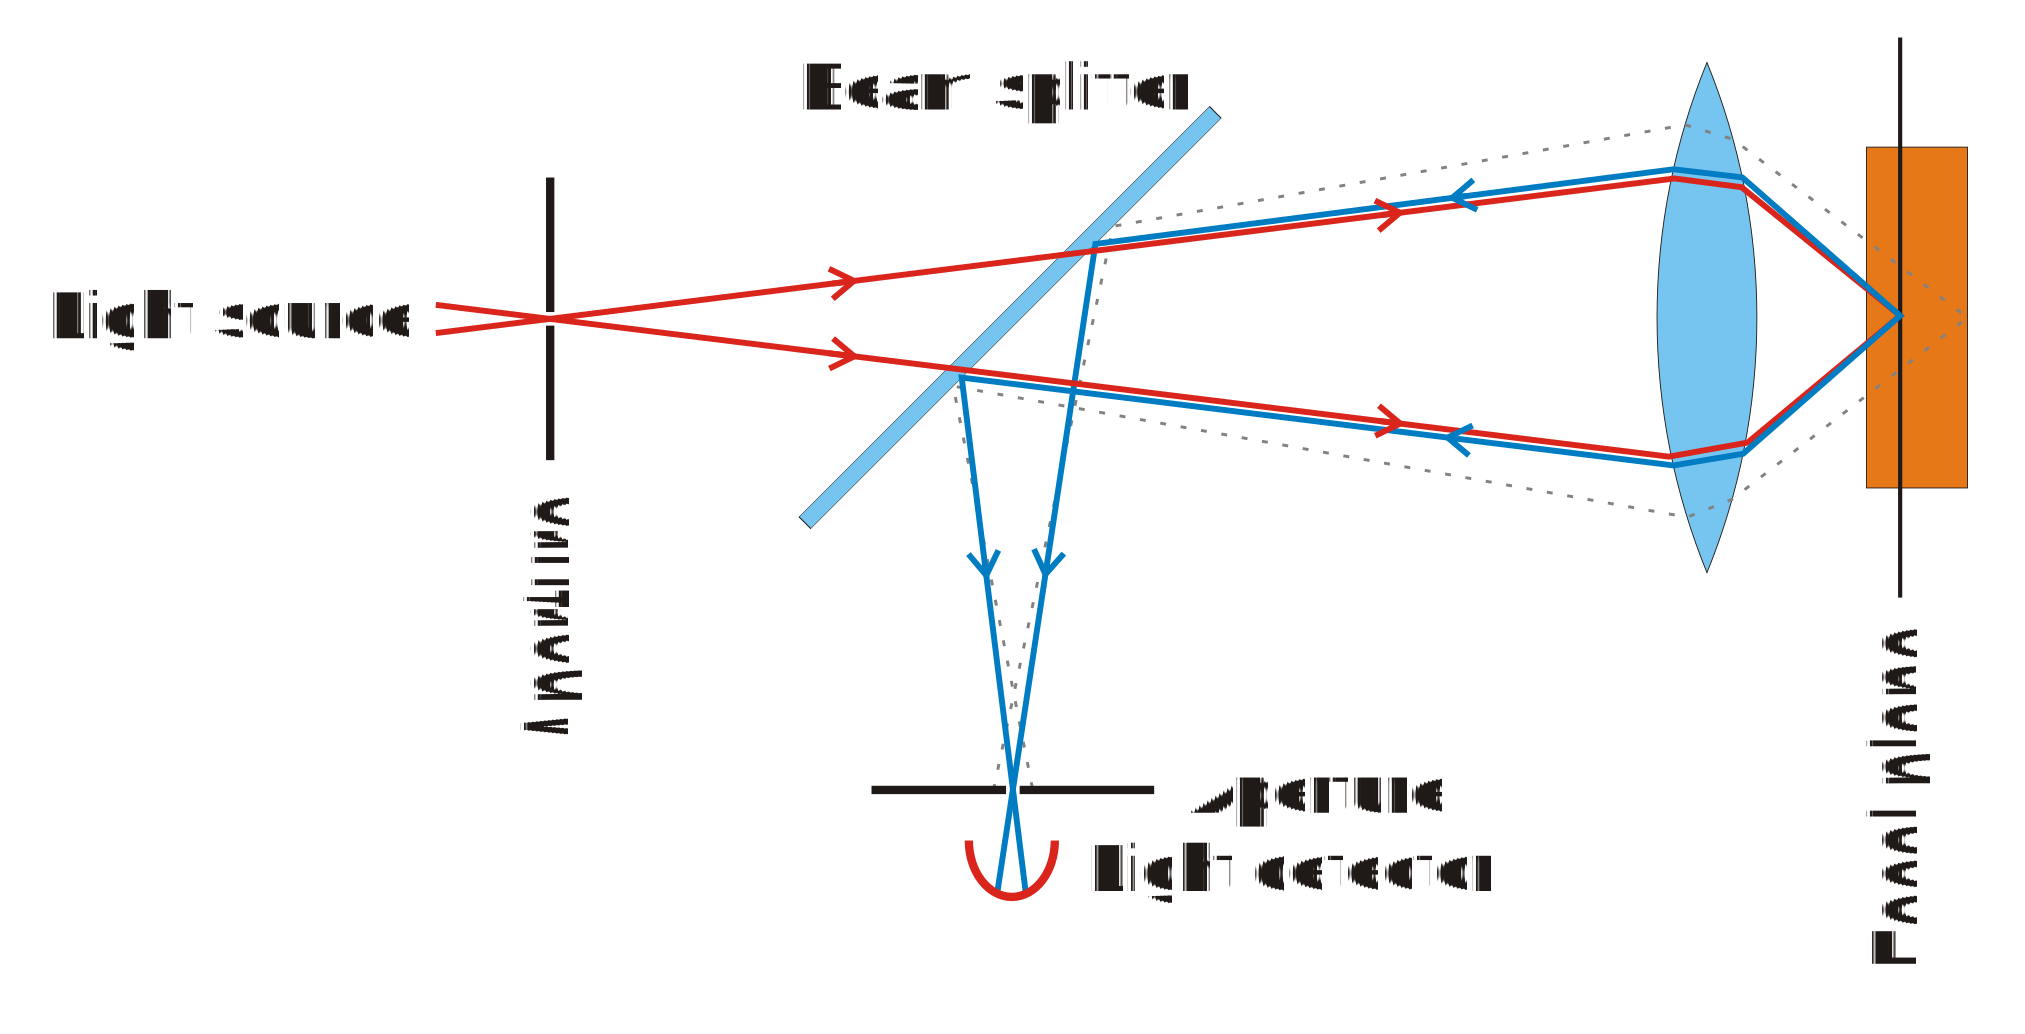
\includegraphics[width=0.95\textwidth]{pictures/ConfocalPrinciple}
\end{center}
\caption{Confocal microscope principle
(source:\href{http://en.wikipedia.org/wiki/File:Confocalprinciple.svg}{Wikipedia
})}
\label{fig:ConfocalPrinciple}
\end{figure}

\begin{figure}[htb]
\begin{center}
\leavevmode
 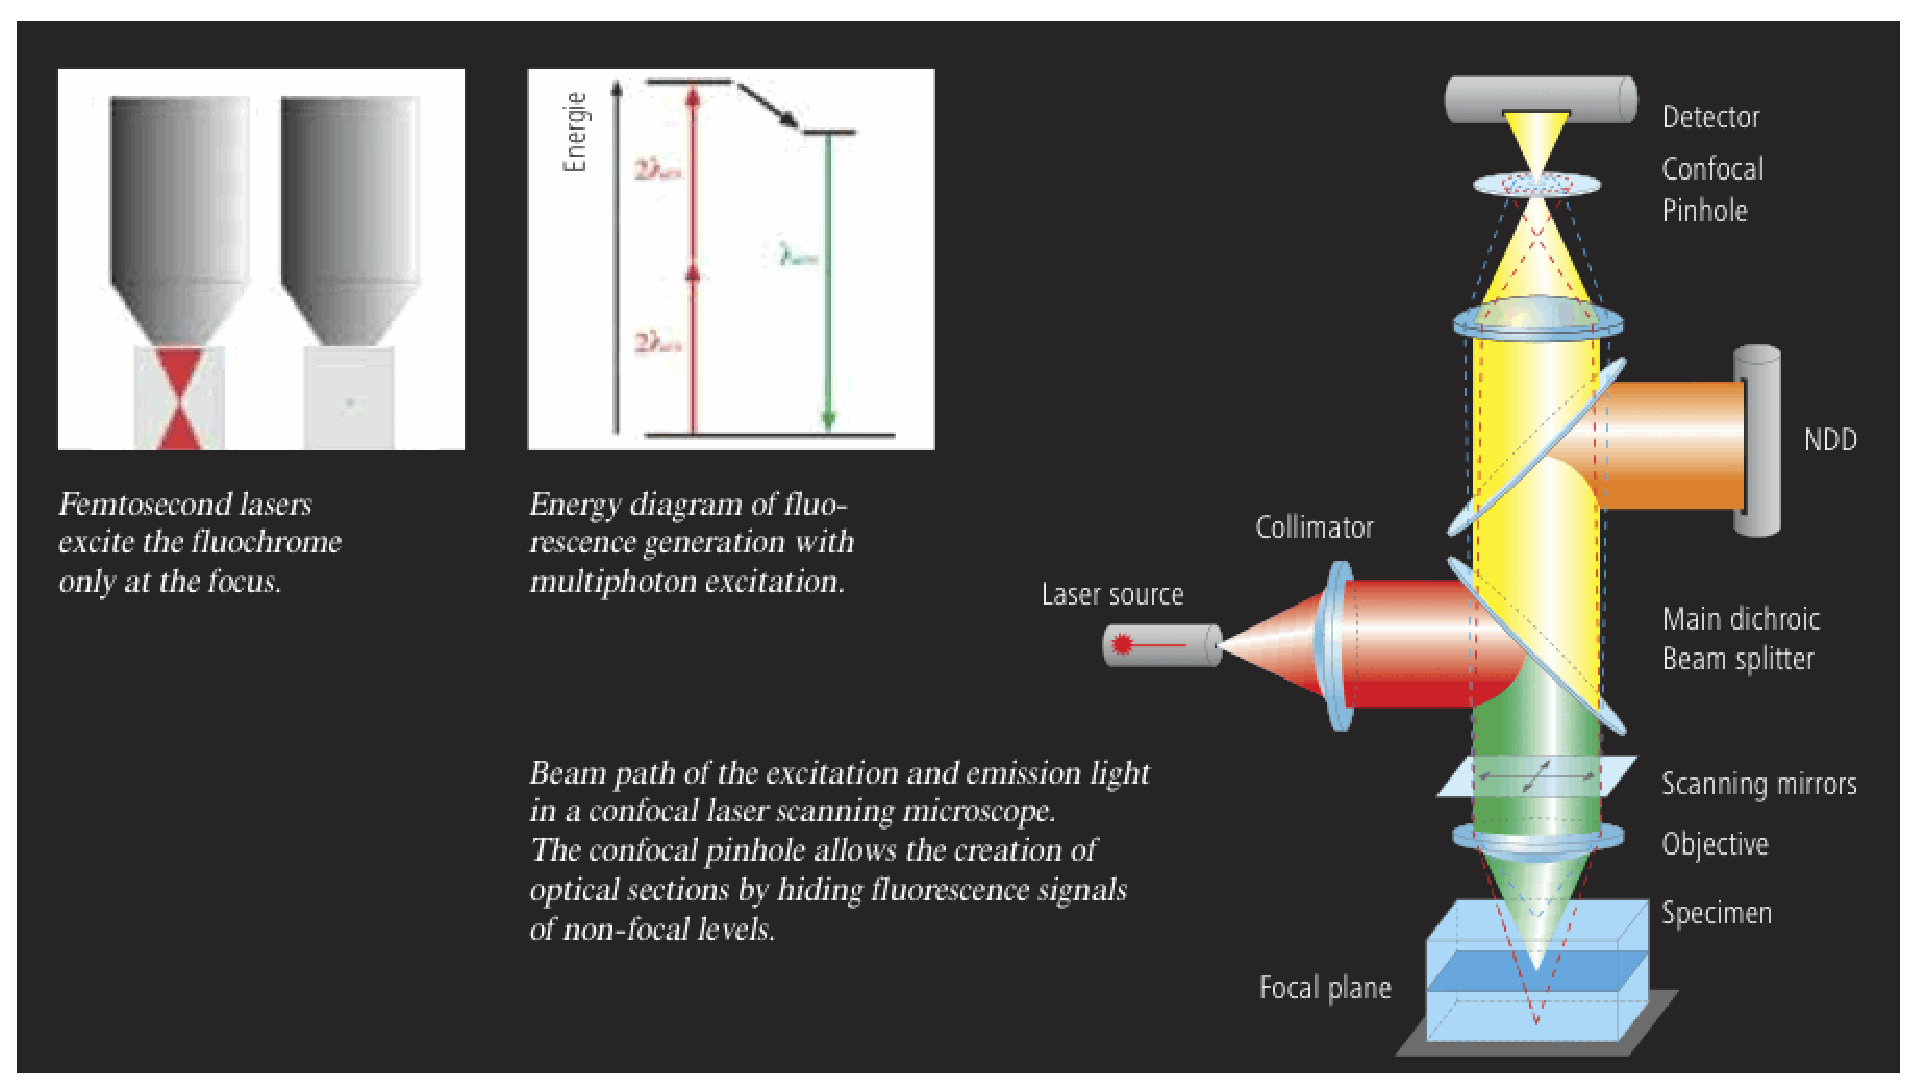
\includegraphics[width=0.95\textwidth]{pictures/ConfocalZeissPrinciple}
\end{center}
\caption{2-photon confocal microscope principle (Zeiss documentation)}
\label{fig:Confocal2photonsPrinciple}
\end{figure}

\begin{figure}[htb]
\begin{center}
\leavevmode
 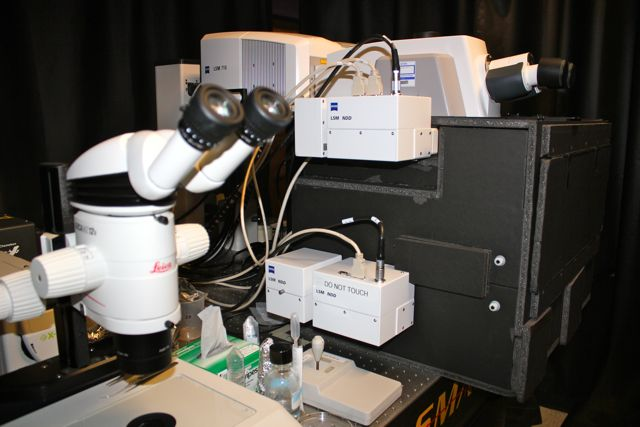
\includegraphics[width=0.95\textwidth]{pictures/PICmicroscope}
\end{center}
\caption{2-photon confocal microscope Zeiss 710 NLO in service in the Megason
Lab}
\label{fig:MicMegason}
\end{figure}

%%%%%%%%%%%%%%%%%%%%%%%%%%%%%%%%%%%%%%%%%%%%%%%%%%%%%%%%%%%%%%%%%%%%%%%%%%%%%%%
%%%%%%%%%%%%%%%%%%%%%%%%%%%%%%%%%%%%%%%%%%%%%%%%%%%%%%%%%%%%%%%%%%%%%%%%%%%%%%%
%%%%%%%%%%%%%%%%%%%%%%%%%%%%%%%%%%%%%%%%%%%%%%%%%%%%%%%%%%%%%%%%%%%%%%%%%%%%%%%

\subsection{Image Processing}

After the embryos have been labelled and imaged, the final challenge of in toto
imaging is image processing. The goal of image processing is to track all the
cell movements and divisions to generate cell lineage trees, to define the
boundaries of all cells and their compartments (nucleus, cytoplasm, membrane,
extracellular space), and to quantize the level of fluorescence within each
cell and subcellular compartment.\\

In order to process all the acquired data, an image processing team of
is working on the next platform of microscopy images analysis: {\gofigure}.
Their goal is to create a very accessible "cross-platform"\footnote{In
computing, cross-platform, or multi-platform, is
an attribute conferred to computer software or computing methods and concepts
that are implemented and inter-operate on multiple operating systems and
hardware.}, "open-source"\footnote{of or
relating to or being computer software for which
the source code is freely available, but which use may be restricted by a
license.}, freely distributed, application with a high quality code, for
biologists to process their data and for computer scientists and image
processing specialists the opportunity to promote their methods.

%%%%%%%%%%%%%%%%%%%%%%%%%%%%%%%%%%%%%%%%%%%%%%%%%%%%%%%%%%%%%%%%%%%%%%%%%%%%%%%
%%%%%%%%%%%%%%%%%%%%%%%%%%%%%%%%%%%%%%%%%%%%%%%%%%%%%%%%%%%%%%%%%%%%%%%%%%%%%%%
%%%%%%%%%%%%%%%%%%%%%%%%%%%%%%%%%%%%%%%%%%%%%%%%%%%%%%%%%%%%%%%%%%%%%%%%%%%%%%%



%
%\begin{figure}[htb]
%\begin{center}
%\leavevmode
%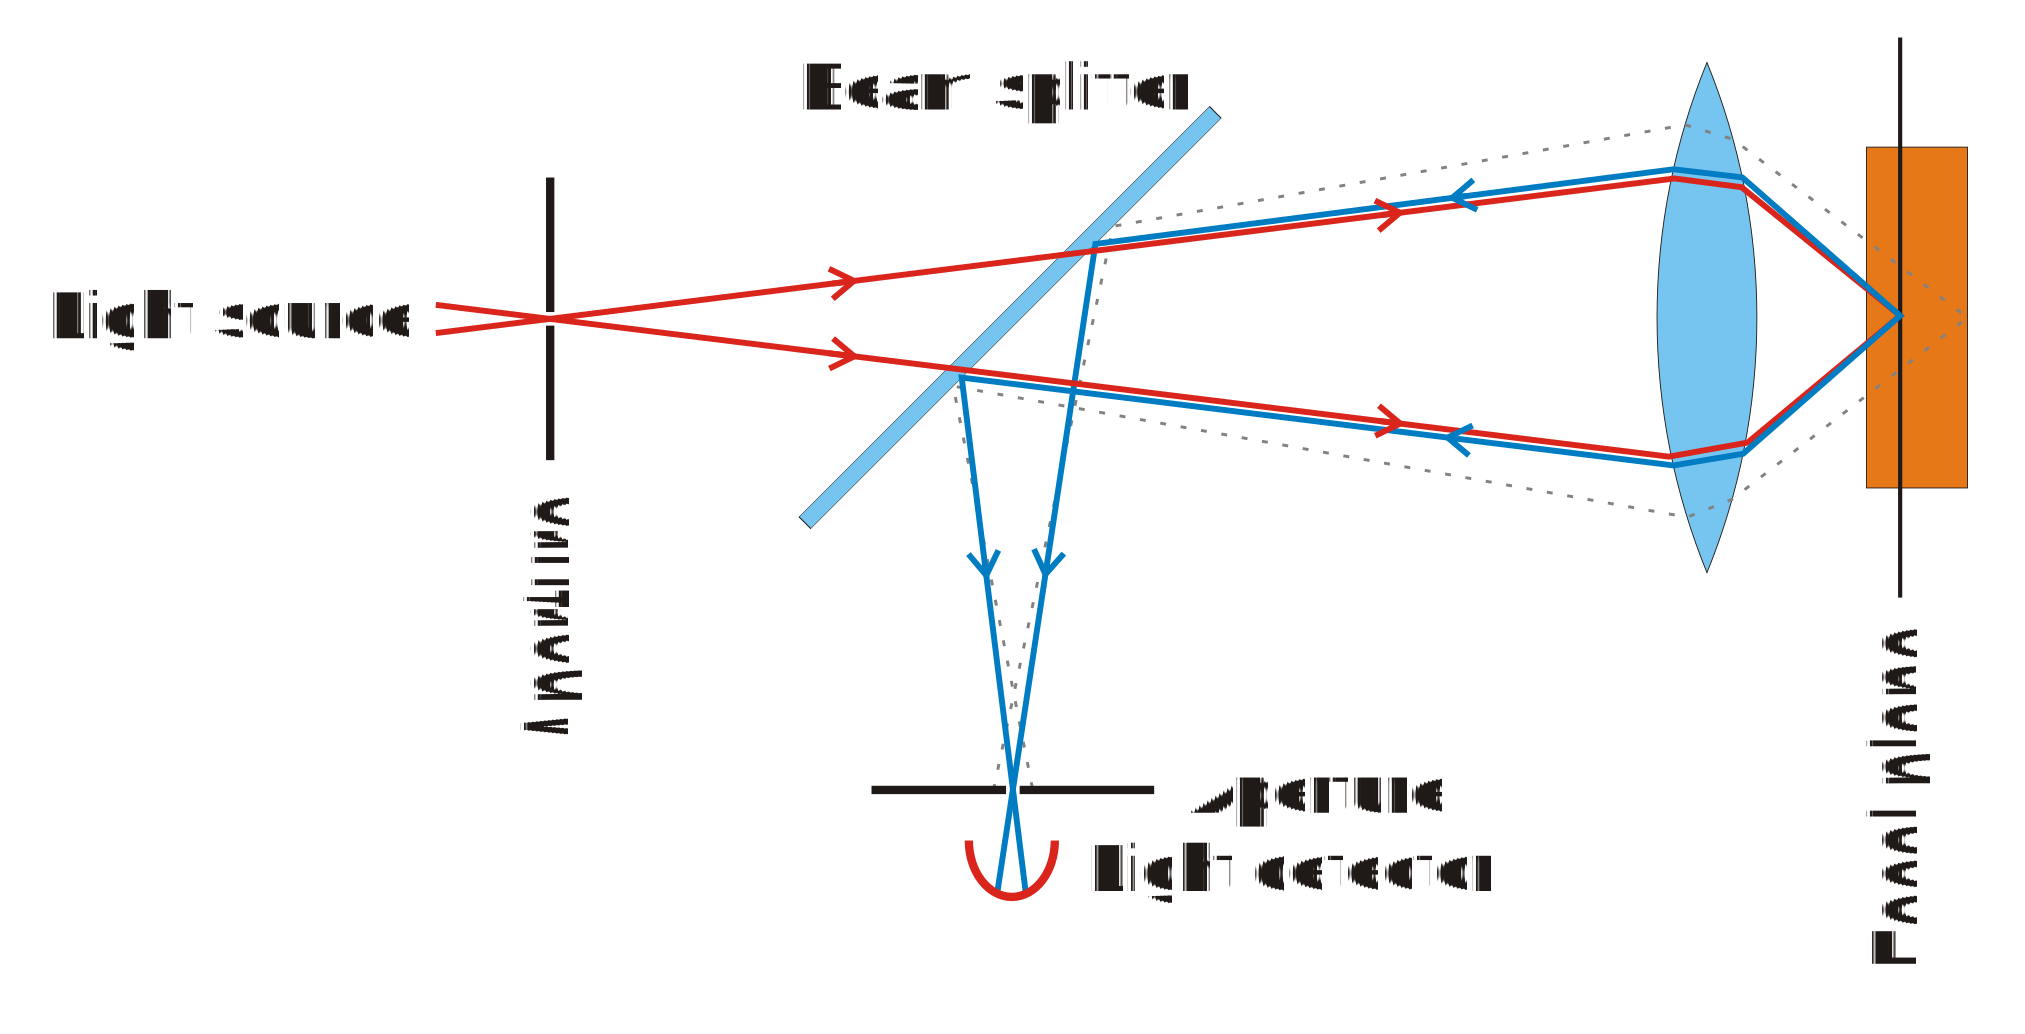
\includegraphics[width=0.95\textwidth]{pictures/ConfocalPrinciple}
%\end{center}
%\caption{Confocal microscope principle (source:\href{http://en.wikipedia.org/wiki/File:Confocalprinciple.svg}{Wikipedia})}
%\label{fig:ConfocalPrinciple}
%\end{figure}
%
%\begin{figure}[htb]
%\begin{center}
%\leavevmode
% 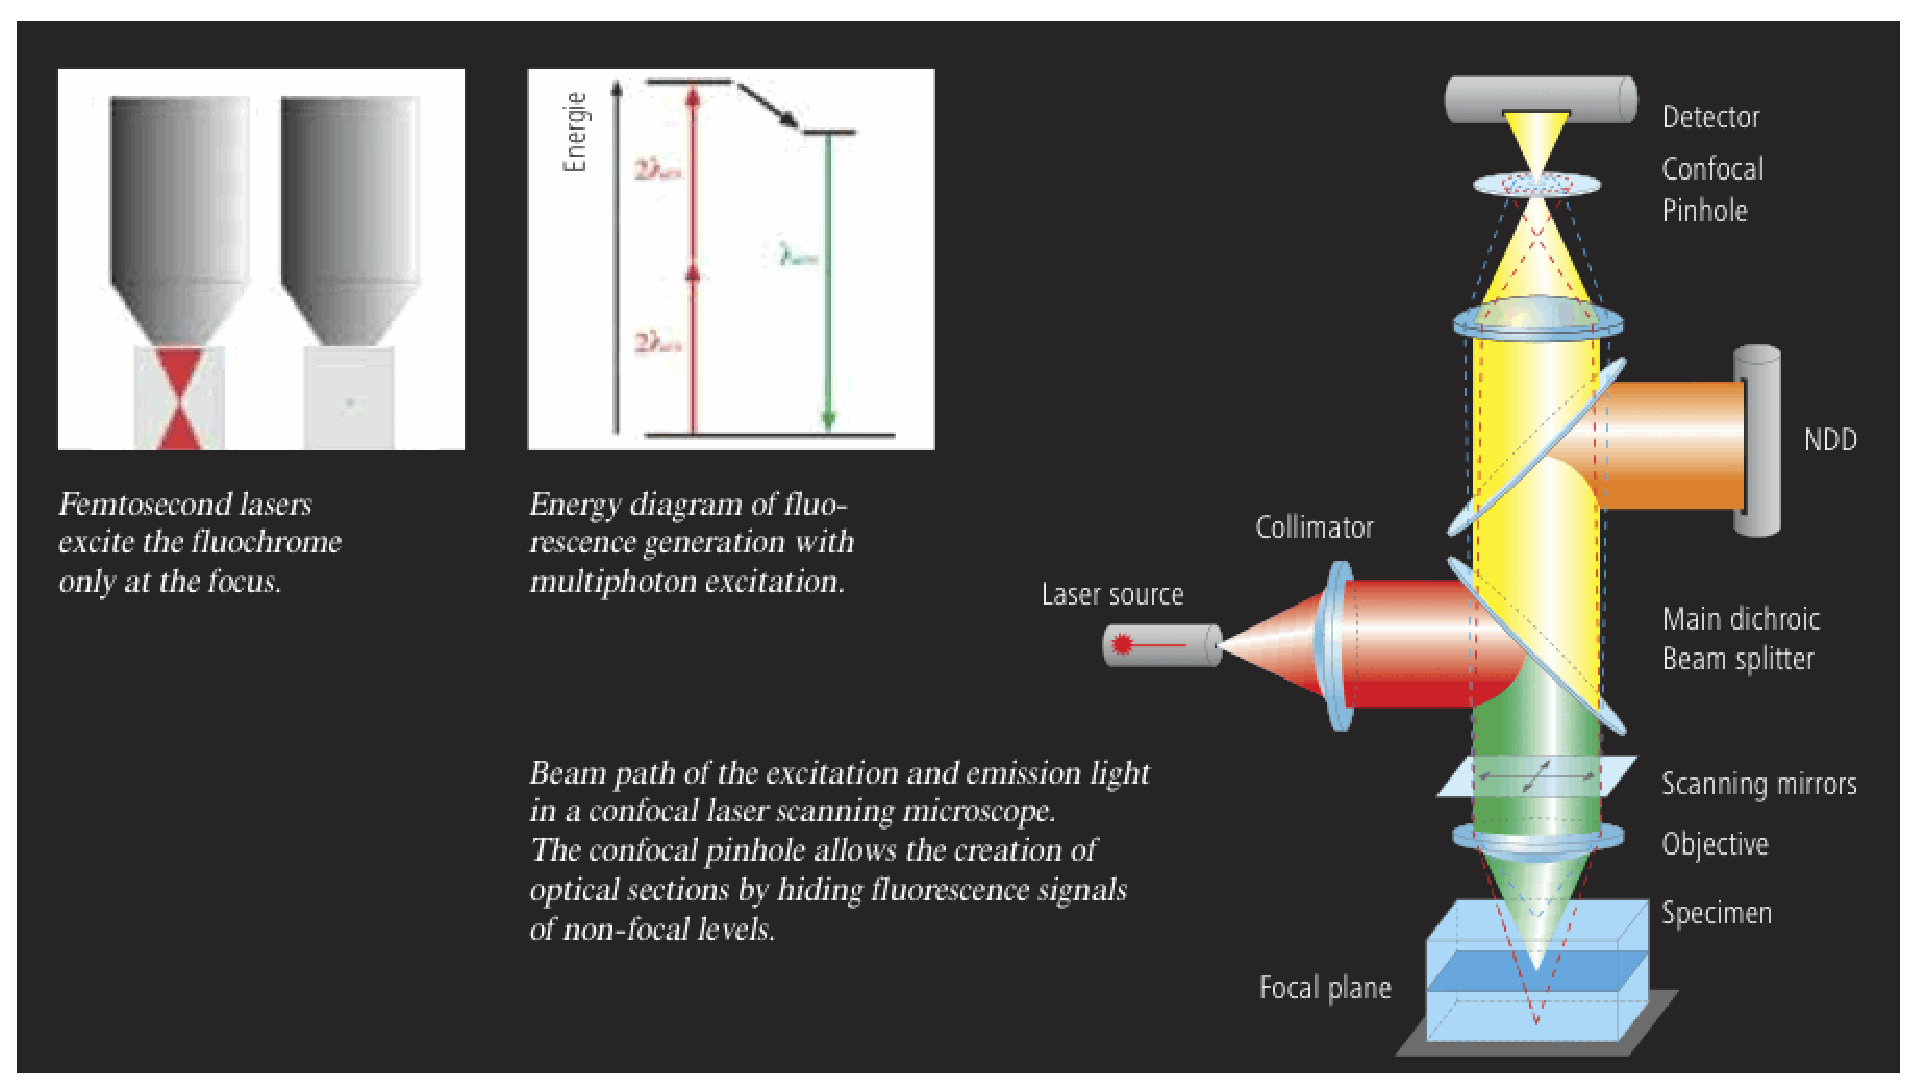
\includegraphics[width=0.95\textwidth]{pictures/ConfocalZeissPrinciple}
%\end{center}
%\caption{2-photon confocal microscope principle (Zeiss documentation)}
%\label{fig:Confocal2photonsPrinciple}
%\end{figure}
%
%\begin{figure}[htb]
%\begin{center}
%\leavevmode
%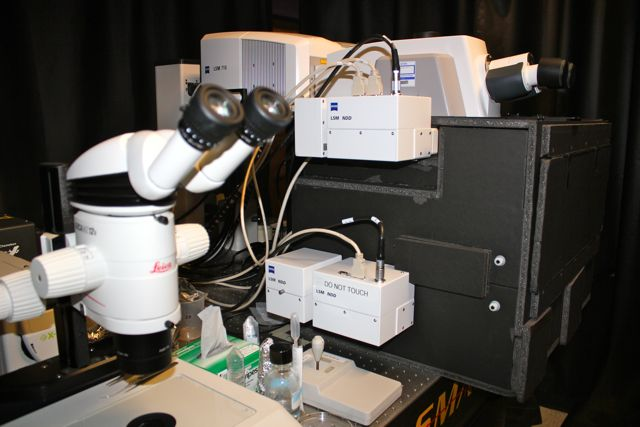
\includegraphics[width=0.95\textwidth]{pictures/PICmicroscope}
%\end{center}
%\caption{2-photon confocal microscope Zeiss 710 NLO in service in the Megason Lab}
%\label{fig:MicMegason}
%\end{figure}

\clearpage



\chapter*{State of the are in the Megason Lab}

The 2-photon/confocal dataset that are prouced in the megason lab, are challenging. They represent a lot of data, and have several artifacts that make image processing much harder.
Even though such confocal datasets are fairly recent, a lot of work has already been done for finding methods to robustly and efficiently process them.
This chapter presents the state of the art in the Megason lab,
namely, the data and techniques that already are available.

%%%%%%%%%%%%%%%%%%%%%%%%%%%%%%%%%%%%%%%%%%%%%%%%%%%%%%%%%%%%%%%%%%%%%%%%%%%%%%%
%%%%%%%%%%%%%%%%%%%%%%%%%%%%%%%%%%%%%%%%%%%%%%%%%%%%%%%%%%%%%%%%%%%%%%%%%%%%%%%
%%%%%%%%%%%%%%%%%%%%%%%%%%%%%%%%%%%%%%%%%%%%%%%%%%%%%%%%%%%%%%%%%%%%%%%%%%%%%%%


\section{Challenges of data sets to be processed}

Biologists acquire tremendous amount of data (see table~\ref{tab:DataSizes})
corresponding in three dimensional videos of zebra fishes embryos
(see figure~\ref{fig:fig:embryoConfocalSlice}).

\subsection{Large amount of data}


We are working on fluorescent microscopy images acquired with a 2-photons confocal microscope. The acquisition process produces huge datasets that we must process efficiently.
Here is a small description of the images :
\begin{figure}[htb]
\begin{center}
\begin{tabular}{|c|c|c|}
\hline Dimension & Size & Resolution \\ 
\hline x (space) & 1024 & 0.24 um \\ 
\hline y (space) & 1024 & 0.24 um \\ 
\hline z (space) & 70 & 1 um \\ 
\hline t (time) & 700 & 2 min\\ 
\hline \multicolumn{3}{|c|}{ 2 intensity channels} \\ 
\hline
\end{tabular} 
\end{center}
\caption{Megason Lab typical fluorescent microscopy dataset}
\label{tab:DataSizes}
\end{figure}
The table~\ref{tab:DataSizes}, shows that the datasets are huge ( the intensity values are coded with {\verb+unsigned char+}, so that a full two channel dataset is approximatively  10.5 Gbit).

Those datasets include nuclei and membrane information in two different intensity channels, and in the future, will include more channels with other biological markers. 


\subsection{Complex data}

The imaging technique is point to point, and a mechanical displacement is involved for moving from on point to another (mirror displacement in the x-y plan, and stage displacement on the z axis). This leads to several artefacts and drawbacks :

\subsubsection{interlacing artefact}
This artefact is due to the microscope's raster scanning: it scans a line, following the x axis, and then increment on the y axis and scans another line.
The uncertainty on the x axis leads to interlacing of successive lines as illustrated figure~\ref{fig:InterlacingArtefact}.
This interlacing is also due to displacement uncertainties while scanning a line : as displacement varies, pixel width varies !
Thus this interlacing artefact is not isotropic: a line may seem to be translated of a positive factor on the right of the image, and of a negative factor on the left !
\begin{figure}[htb]
  \centering
  \subfloat[nuclei channel]{\label{fig:InterlaceNuclei}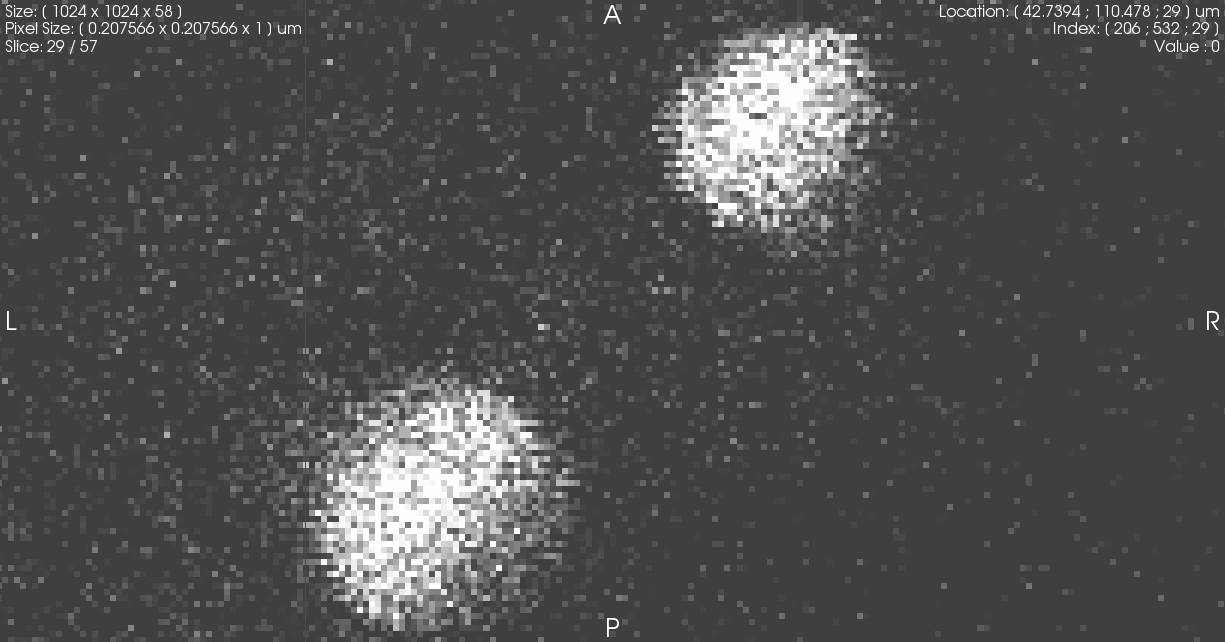
\includegraphics[width=0.7\textwidth]{pictures/InterlacingNuclei}}\\
  \subfloat[membrane channel]{\label{fig:InterlaceMembrane}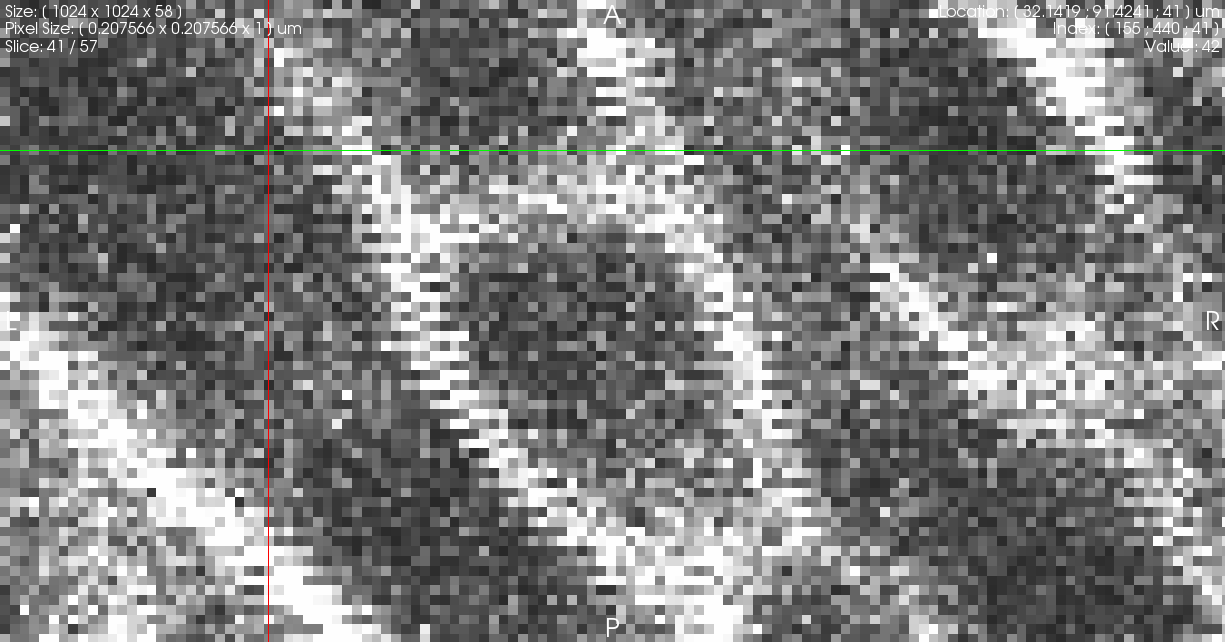
\includegraphics[width=0.7\textwidth]{pictures/InterlacingMembrane}}                
  \caption{Interlacing artefact on 2 photon confocal images. Views are x-y cuts of a 3D volume}
  \label{fig:InterlacingArtefact}
\end{figure}


\subsubsection{Anisotropy of images}

The datasets acquired in the Megason lab are anisotropic. As in the medical imaging domain, specialists are used to analyse images "slice by slice"
instead of considering them as a volume. They are worried about having a very detailed image in the x-y plan, and don't really worry about the other dimension.
This way of seeing things is wrong for images processing. A completely anisotropic image is very hard to process.
Non existing structures appear in the third dimension as illustrated figure~\ref{fig:anisotropy}.
If a human brain with its understanding of the data may be able to interpret these structures, they lead most common algorithms to failure.
We can notice that nuclei seem to be stuck together and membrane's closure is almost always missing. This gives challenging a priori introduction problems.

Another challenging problem comes from inhomogeneous intensity as described in~\cite{umesh2001efficient}, along the z axis (see figure~\ref{fig:membraneHolesXZ}).
\begin{figure}[htb]
  \centering
  \captionsetup[subfloat]{labelformat=empty}
  \subfloat[][]{{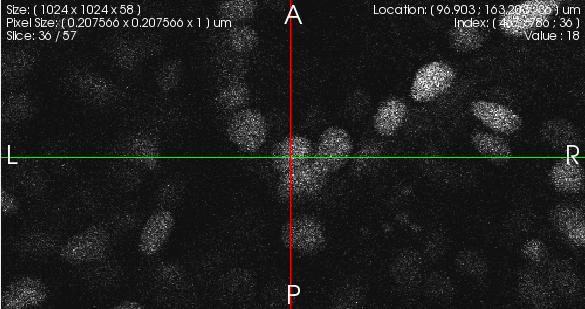
\includegraphics[width=0.7\textwidth]{pictures/anisotropieNucleiXY}\label{fig:anisotropieNucleiXY}}}\\
  \subfloat[][]{{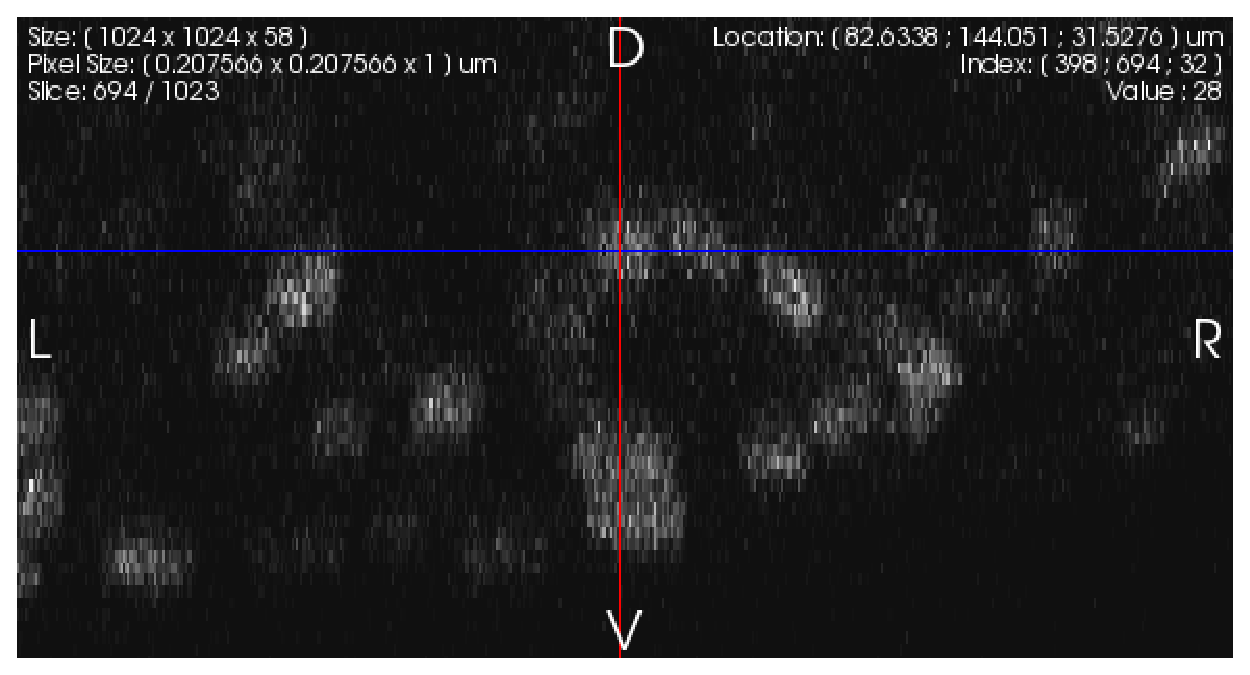
\includegraphics[width=0.7\textwidth]{pictures/anisotropieNucleiXZ}\label{fig:anisotropieNucleiXZ}}}
\caption{%
Illustration of the anisotropy of the datasets in the nuclei channel (view along xy~\subref{fig:anisotropieNucleiXY}, along xz~\subref{fig:anisotropieNucleiXZ}).}
\label{fig:anisotropy}
\end{figure}
\begin{figure}[htb]
  \centering
  \captionsetup[subfloat]{labelformat=empty}
  \subfloat[][]{{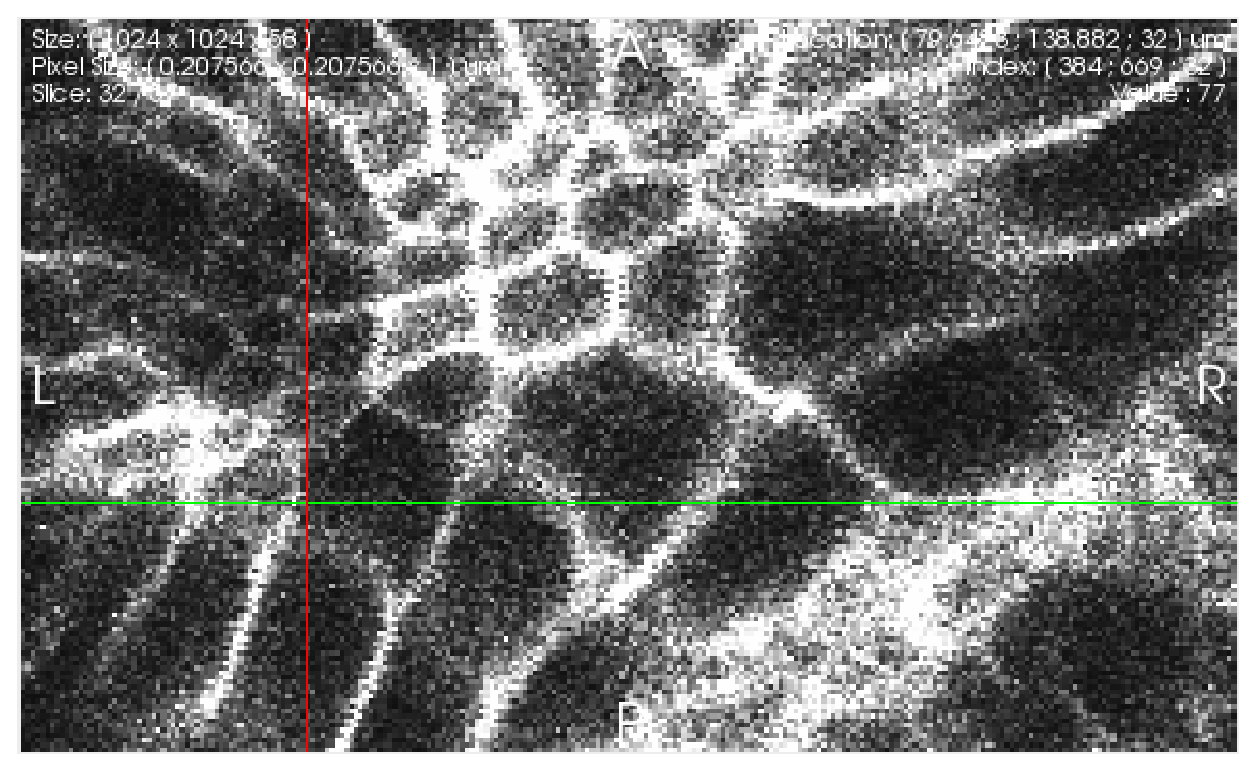
\includegraphics[width=0.7\textwidth]{pictures/anisotropieMembraneXY}\label{fig:anisotropieMembraneXY}}}\\
  \subfloat[][]{{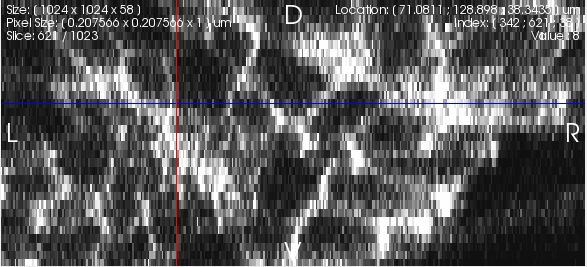
\includegraphics[width=0.7\textwidth]{pictures/anisotropieMembraneXZ}\label{fig:anisotropieMembraneXZ}}}
\caption{%
Illustration of the anisotropy of the datasets in the membrane channel (view along xy~\subref{fig:anisotropieMembraneXY}, along xz~\subref{fig:anisotropieMembraneXZ})}
\label{fig:anisotropy}
\end{figure}

\subsubsection{Noise}

There is much noise present in the datasets (see figure~\ref{noiseNuc}). Both membrane channel and nuclei channel are populated with non Gaussian noise.
The noise comes both from the microscope and electronics acquisition equipments, and from the biological sample that can be fluorescent in random locations.
The acquisition noise along z axis is decorrelated.
\TODO{get histograms of noise}
The problem also comes from the fact that depending on the phosphor used, the noise's statistics will differ.
\begin{figure}[htb]
\centering
  \subfloat[][]{{
\includegraphics[width=0.3\textwidth]{pictures/noiseXY}\label{fig:noiseXY}}} \hspace{5pt}
  \subfloat[][]{{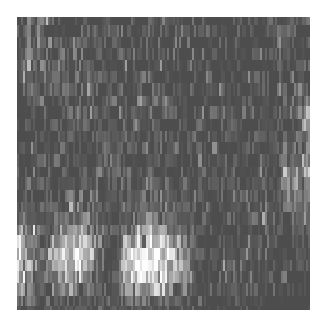
\includegraphics[width=0.3\textwidth]{pictures/noiseXZ}\label{fig:noiseXZ}}}
  \caption{%
    Illustration of the noise in the nuclei channel of confocal images.
    \subref{fig:noiseXY}: in a xy slice;
    \subref{fig:noiseXZ}: in a xz slice. 
    Notice, that \subref{fig:noiseXY} contains some nuclei as references, in the top right corner, and \subref{fig:noiseXZ} in the bottom left.}
\label{fig:noiseNuc}
\end{figure}


\subsubsection{Low resolution of images}

The imaging process, combined with a too low resolution, leads to merged or missing structures. The nuclei channel displays very often clusters of merged nuclei (see figure~\ref{fig:anisotropy}) when the membrane channel has information holes (see figure~\ref{fig:holesMembrane}.
\begin{figure}[htb]
  \centering
  \captionsetup[subfloat]{labelformat=empty}
  \subfloat[][]{{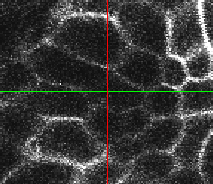
\includegraphics[width=0.45\textwidth]{pictures/membraneHolesXY}\label{fig:membraneHolesXY}}}\hspace{5pt}
  \subfloat[][]{{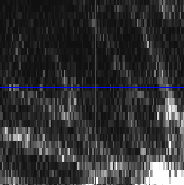
\includegraphics[width=0.45\textwidth]{pictures/membraneHolesXZ}\label{fig:membraneHolesXZ}}}
%\subfloat[][]{{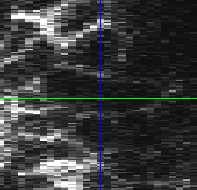
\includegraphics[width=0.7\textwidth]{pictures/membraneHolesYZ}\label{fig:membraneHolesYZ}}}
\caption{%
Illustration of missing information in the membrane channel. Holes and intensity inhomogeneities in a xy plan~\subref{fig:membraneHolesXY}, a xz plan~\subref{fig:membraneHolesXZ}.}
\label{fig:holesMembrane}
\end{figure}


\subsubsection{Point spread function}

The impulse response of the microscope is a noisy point spread function (see figure~\ref{fig:pointSpreadPrinciple}).
That adds a deconvolution problem that can be treated together with the denoising problem.
For simplicity reasons, researchers image with a very low resolution along the z axis, as the impulse function is spread out a lot along this axis.
It is possible to correct such noise by knowing the impulse response of the microscope.
Knowing exactly this PSF, would give us the chance to have a better z resolution, by oversampling in z, and deconvolving.
For that purpose, we could image a sub-pixelic fluorescent object, and evaluate the impulse response of the whole system.
\begin{figure}[htb]
\begin{center}
\leavevmode
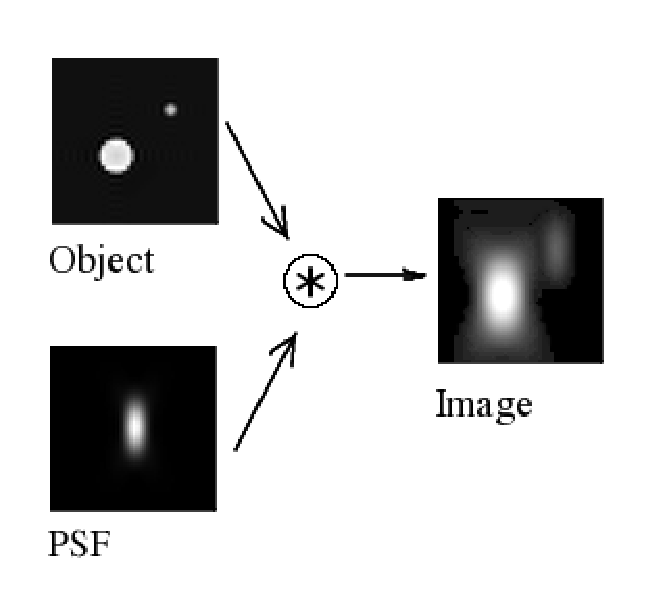
\includegraphics[width=0.5\textwidth]{pictures/pointSpreadFunction}
\end{center}
\caption{Illustration of the Point Spread Function (PSF) principle : the object is convoluted with the PSF.}
\label{fig:pointSpreadPrinciple}
\end{figure}


\subsubsection{Complex structures}

The images we get are complex assembly of cells.
Some area being full of membrane, and others full with inter cellular liquid.
This is not a simple microscope slide with some well known cells, but a whole developing organism.


%%%%%%%%%%%%%%%%%%%%%%%%%%%%%%%%%%%%%%%%%%%%%%%%%%%%%%%%%%%%%%%%%%%%%%%%%%%%%%%
%%%%%%%%%%%%%%%%%%%%%%%%%%%%%%%%%%%%%%%%%%%%%%%%%%%%%%%%%%%%%%%%%%%%%%%%%%%%%%%
%%%%%%%%%%%%%%%%%%%%%%%%%%%%%%%%%%%%%%%%%%%%%%%%%%%%%%%%%%%%%%%%%%%%%%%%%%%%%%%

\section{The Megason lab imaging pipeline}

Dr Kishore Mosaliganti has been working for two years in the Megason lab, in order to develop new segmentation methods for fluorescent images.
He has been working on experiencing and developing diverse algorithms for nuclei and membrane detection and segmentation.
As presented is the previous section, the datasets in the Megason Lab are extremely challenging:
they are huge and present important drawbacks (resolution, noise) as they are provided for visual processing and not computer assisted processing.

As these datasets are very big, and four dimensional, it is not possible to use Matlab for easy prototyping and experiencing : 
most of the time, the very low resolution third dimension will considerably modify the results.
There is also a time issue : the datasets must be treated in an acceptable amount of time,
and that prevents us from using Matlab language that does not provide every optimized function that we need for 3D images visualization and processing.
This forces us to program and prototype in {\C++}. The standard library used for image processing in the Megason Lab is ITK. Kishore's algorithm are all coded with this library.
The data processing in ITK is represented by pipelines : a series of connected filters that perform image processing tasks.
The Megason lab aslo develops a visualization program for microscopy data: {\gofigure}. This program uses ITK and VTK for processing and visualization of data. The long term goal being to include the algorithms to {\gofigure}, we also have to use those libraries.

Kishore studied several pipelines for nuclei and membrane segmentation.
For nuclei segmentation, an approach based on detection of nuclei, and region growing with the level set theory was used last year.
This year, a new approach based on nuclei detection and watershed algorithms is being used.
The algorithm used are standard and contour based for the detection of nuclei.
This leads to many errors in detection, due to the poor image quality. Right now, these errors are compensated after the segmentation step.

For membrane segmentation, Kishore is proposing a very good denoising technique based on anisotropic diffusion and tensor voting.
The reconstruction of the membrane structure is effective, even in low quality images. A segmentation step has to be implemented on top of it.
